\documentclass[12pt]{report}
\usepackage[utf8]{inputenc}
\usepackage[a4paper,width=150mm,top=25mm,bottom=25mm]{geometry}
\usepackage{graphicx}

\usepackage{fancyhdr}
\pagestyle{fancy}

\newcommand{\thtitle}{Smooth Curve Geometry}
\newcommand{\thsubtitle}{On The Geometric Tangent Structure of a Smooth Manifold and Its Calculus}
\newcommand{\thauthor}{Marcelo Guimarães Neto}

\fancyhead[R]{\rightmark}
\fancyhead[L]{}

\usepackage{biblatex}
% \usepackage[style=alphabetic]{biblatex}
\addbibresource{references.bib}

\usepackage{lipsum}

\graphicspath{{\images}}

% Available document structure commands:

% Book: \part{}, \chapter{}, \section{}, \subsection{}, \subsubsection{}, \paragraph{}, \subparagraph{}.

% Report: \part{}, \chapter{}, \section{}, \subsection{}, \subsubsection{}, \paragraph{}, \subparagraph{}.

% Article: \part{}, \section{}, \subsection{}, \subsubsection{}, \paragraph{}, \subparagraph{}.

\begin{document}

\begin{titlepage}
    \begin{center}
        % \vspace*{1cm}
            
        \Huge
        \textbf{\thtitle}
            
        \vspace{0.5cm}
        \LARGE
        \thsubtitle  
        
		\vspace{1cm}
        \Large    
        Author: \textbf{Marcelo Guimarães Neto}
		
		Supervisor: \textbf{Konstantin Izyurov}

        \vfill
        A thesis presented for the degree of\\
        Bachelor of Science
            
        \vspace{0.8cm}
        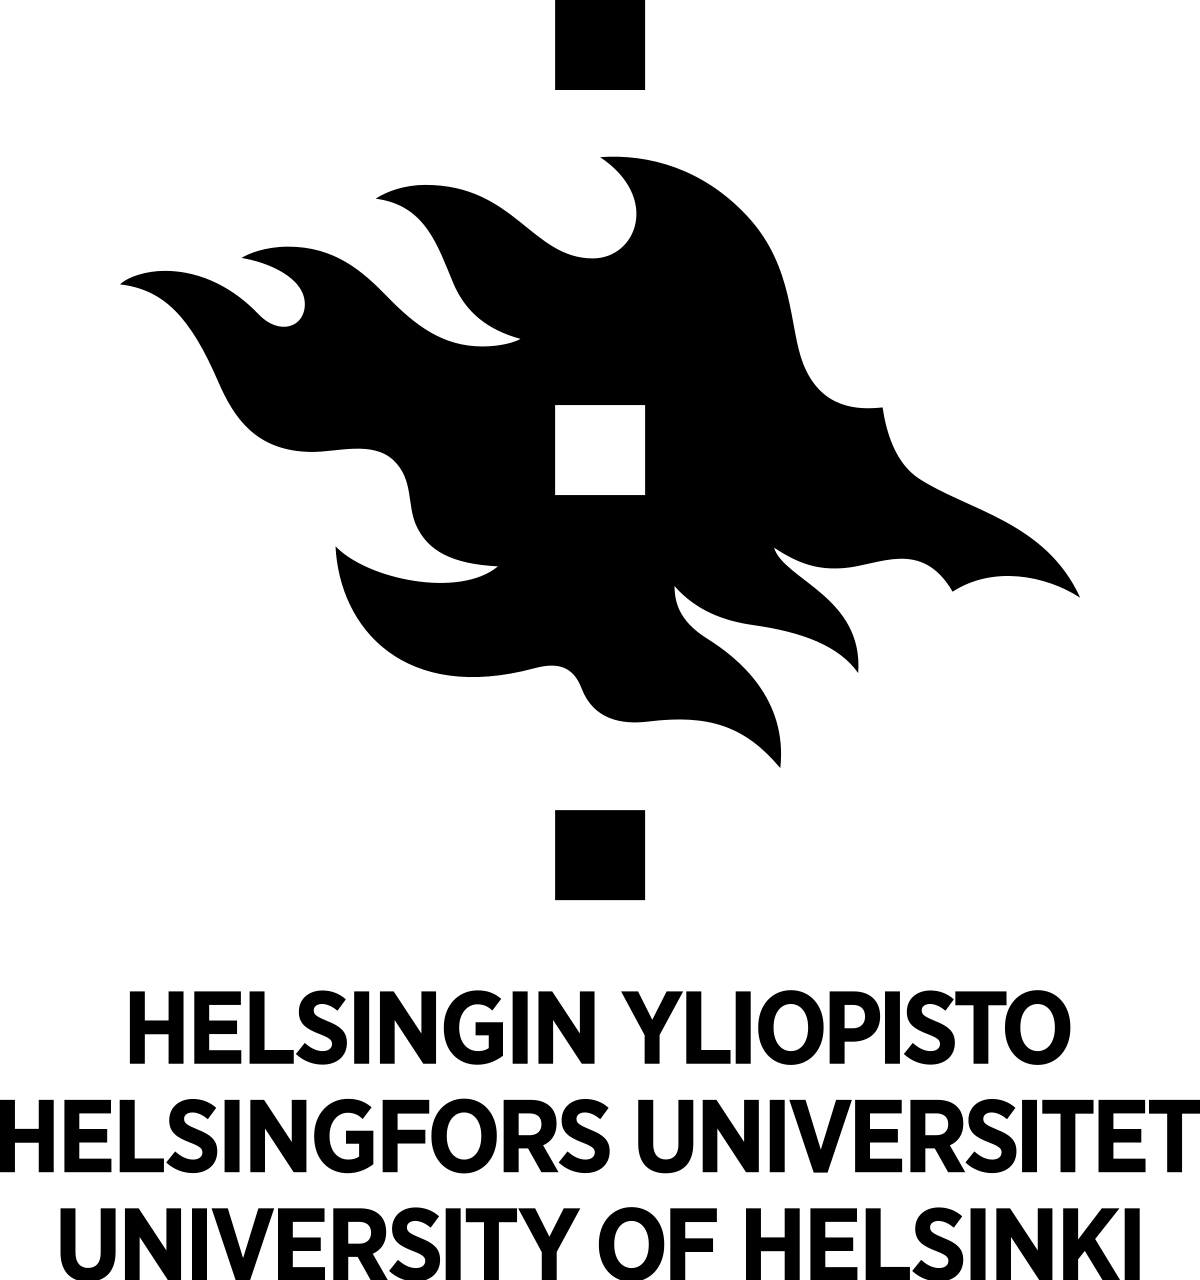
\includegraphics[width=0.4\textwidth]{heluni-logo.png}
        
        \vspace{0.8cm}
        Department of Mathematics and Statistics\\
        Faculty of Science\\
        University of Helsinki\\
        Finland\\
        \today
            
    \end{center}
\end{titlepage}


\thispagestyle{plain}
\begin{center}
    \Large
    \textbf{The Even Subalgebras of Euclidean Geometric Spaces}
        
    \vspace{0.4cm}
    \large
    A Geometric Proof of the Frobenius Classification of Finite-Dimensional Associative Division Algebras over the Reals       

    \vspace{0.4cm}
    \textbf{Marcelo Guimarães Neto}
       
    \vspace{0.9cm}
    \textbf{Abstract}
\end{center}
Lorem ipsum dolor...


\chapter*{Acknowledgements}
I want to thank...

\tableofcontents
\listoffigures
\listoftables

\chapter{Introduction}
\section{Historical Background}
\lipsum[4-5]

\section{Motivation}
\lipsum[2-5]

\chapter{Mathematical Background}
\section{Abstract Algebra: A Brief Primer}

\subsection{Modules and Vector Spaces}
\lipsum[3-5]

\subsection{Algebras}
\lipsum[3-5]

\section{Set Theoretic Topology: Select Topics}

\subsection{(Co-)Induced, Product and Quotient Topologies}
\lipsum[3-5]

\subsection{Topological Manifolds}
\lipsum[3-5]

% CONTENT BELOW IS REDUNDANT AND SHOULD ACTUALLY GO IN THE MAIN BODY

% \section{Analysis on Vector Spaces and Algebras}

% \subsection{Topology: Banach and Hilbert}
% \lipsum[1-5]
% \cite{einstein}

% \lipsum[2-5]

% \subsection{Differentiation}
% \lipsum[3-5]

% \subsection{Measure and Integration}
% \lipsum[3-5]

% \section{Differential Geometry}

% \subsection{Topological Manifolds}
% \lipsum[1-5]
% \lipsum[1-5]

% \subsection{Tangent Structure}
% \lipsum[1-5]
% \cite{latexcompanion}
% \lipsum[1-5]

% \subsection{Connections, Covariant Derivatives and Differential Forms}
% \lipsum[1-5]
% \cite{latexcompanion}
% \lipsum[1-5]

% \subsection{(Pseudo-)Metric Structure}
% \lipsum[2-5]

\chapter{Geometric Algebra}
\section{The Axioms}

\section{The Elements}

\section{The Products}


\chapter{Geometric Calculus}

\section{Analysis on Geometric Algebras}

\subsection{Topology: Banach and Hilbert}
\lipsum[1-5]
\cite{einstein}

\lipsum[2-5]

\subsection{Differentiation}
\lipsum[3-5]

\subsection{Measure and Integration}
\lipsum[3-5]

\section{Differential Geometry}

\subsection{Topological Manifolds}
\lipsum[1-5]
\lipsum[1-5]

\subsection{Geometric Tangent Structure}
\lipsum[1-5]
\cite{latexcompanion}
\lipsum[1-5]

\subsection{Connections, Covariant Derivatives and Differential Forms}
\lipsum[1-5]
\cite{latexcompanion}
\lipsum[1-5]

\subsection{(Pseudo-)Metric Structure}
\lipsum[2-5]

\chapter{Conclusion}
In this paper, we have developed the fundamentals of Geometric Algebra.

Starting from a formal set of axioms, we have thoroughly derived the general properties of the algebra, its elements and its products.

We have observed that the algebra does indeed encompass the algebra of the real and complex numbers and that of the quaternions, with the marked advantage of naturally generalizing to higher dimensions.

Geometric Algebra - and its extension to the domain of analysis, Geometric Calculus - have many promising applications that unfortunately were outside the scope of this thesis: linear and multilinear algebra can be expressed in the language of frames and outermorphisms; differential geometry can be formulated in the framework of vector manifolds and the geometric derivative with the promise of coordinate-free computations; the even subalgebras of Euclidean geometric spaces can be shown to account for the theory of Spinors; advances have even been made in the theory of Lie Algebras and Groups.

\textbf{Geometric Algebra} postulates that geometry is a fundamental guide towards meaningful mathematical pursuits, even in abstract settings. It should be no surprise that such a theory would be so adept at describing a wide range of geometric phenomena. As \textit{Hestenes} puts it \cite[p. xii]{ga-origin}:
\begin{quote}
	``Geometry without algebra is dumb! Algebra without geometry is blind!''
\end{quote}




\appendix
\chapter{Topological Manifolds as Curve Bundles}
\input{appendix/curve-bundles}

\printbibliography

\end{document}
